\chapter{Solution}
\label{ch:Model}

% We [outline|describe|introduce] our [proposed] [solution|model], [justify] design decisions and [implementation details| detail implementation| document implementation details].
In this chapter, we describe our experiments, justify design decisions and detail our implementation. A high-level overview of our solution is provided in Fig.~\ref{fig:overview}. 
\begin{figure}[ht]
	\centering
	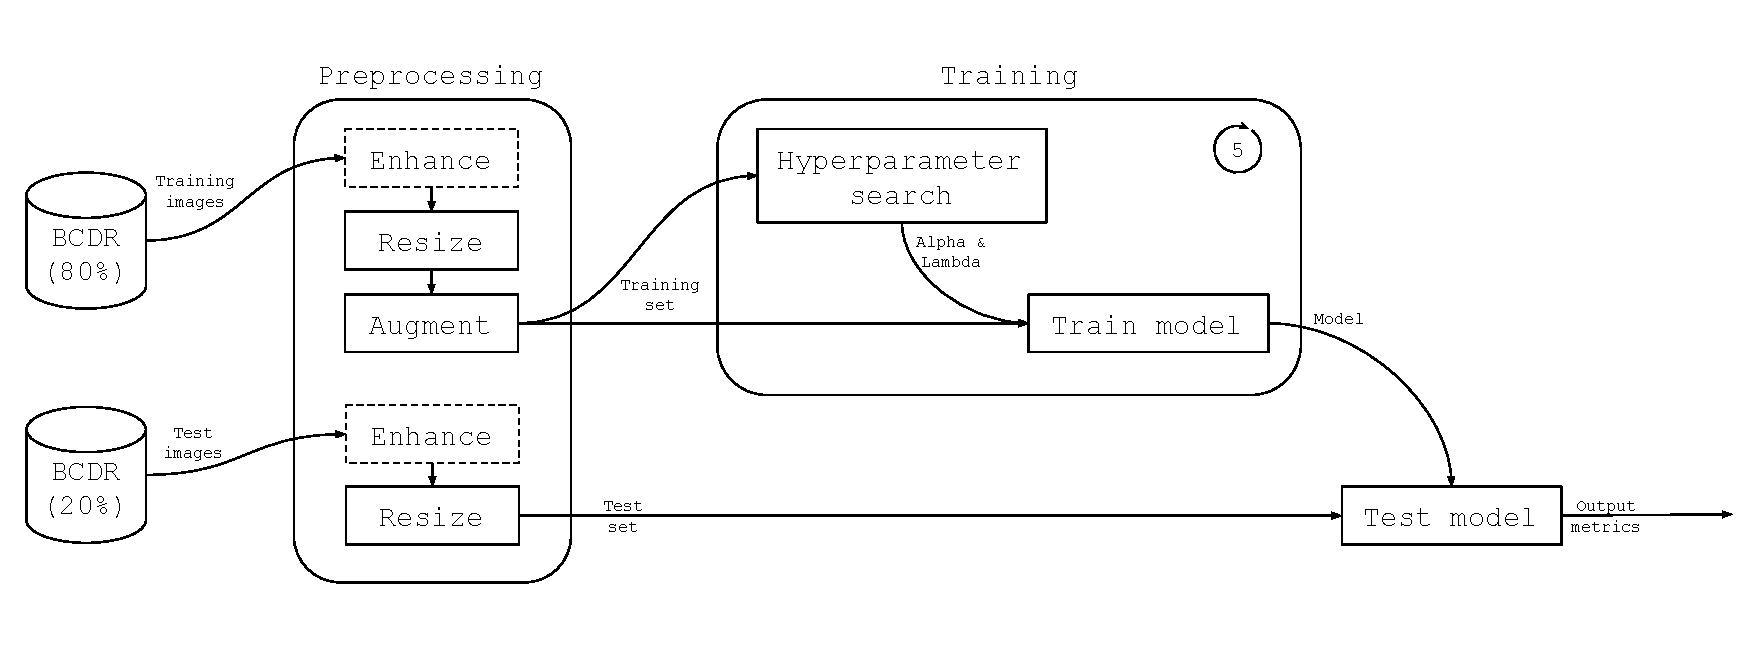
\includegraphics[width=\textwidth]{plots/overview.pdf}
	\caption[Overview of the solution]{Overview of our solution. We divide the database into training and test patients, train a convolutional network with the training set (we select hyperparameters $\alpha$ and $\lambda$ using 20\% of the training set for validation) and evaluate our model in the test set. We repeat each experiment for five folds. Experiments test different preprocessing and network configurations.}
	\label{fig:overview}
\end{figure}

\section{Task definition}
We segment digital mammograms into two separate regions: breast mass (benign or malignant) and general tissue.
Breast area is previously separated from the background by simple thresholding.
In particular, we train a convolutional network to estimate the probability of each pixel belonging to a mass and evaluate these predictions.

\section{Data set}
%We document the retrieval, enhancement, labelling and augmentation of [the|our] data set [used for the experiments].
% We document how we retrieve, enhance, label and augment our data set.
We document the retrieval, enhancement and augmentation of our data set.

\subsection{Database}
We use the Breast Cancer Digital Repository (BCDR-DM) database, specifically, the BDCR-D01 data set, which is composed of patients with at least one breast mass.
%We curated it to delete patients with breast implants.
We select 256 digital mammograms from 63 patients.
A patient with breast implants (511) was ignored.
Digital mammograms have higher image quality and lack any marks or scanning artifacts present in digitized film mammograms; this allows the network to learn sharper features easying segmentation.
We overcome having few mammograms at our disposal by augmenting our data set and training on overlapping patches.

Mammograms in the BCDR-D01 data set are 8-bit grayscale images with 0.07mm spatial resolution sized $3328\times 4084$, $2816\times 3072$ or $2560 \times 3328$ pixels equivalent to $23.3 \times 28.6$, $19.7 \times 21.5$ and $17.9 \times 23.3$ centimeters.
%Each lesion's segmentation, type (mass, microcalcification, calcification, axillary adenopathy, architectural distortion or stroma distortion) and biopsy result (benign or malignant) are provided.
The data set provides the segmentation, type (mass, microcalcification, calcification, axillary adenopathy, architectural distortion or stroma distortion) and biopsy result (benign or malignant) of each lesion.
%Segmentation, type and biopsy result for each lesion are provided. 
%Each lesion is segmented and its type (mass, microcalcification, calcification, axillary adenopathy, architectural distortion or stroma distortion) and biopsy result (benign or malignant) are supplied.
We disregard patient data (age and breast density) and image features (intensity, texture, shape and location descriptors).
%do not make use of/employ/ ignore/disregard

We generate our labels thresholding the mammogram to zero to separate the background and using the provided lesion outlines to separate the lesions.
%and separating the background by thresholding to zero. 
%Labels were generated using the provided outlines and thresholding the background to zero.
Masses (benign or malignant) appear as white; breast area as gray and background as black (Fig.~\ref{subfig:Preprocessinga}).

\subsection{Data division}
For each fold, we randomly assign 80\% of patients to the training set and 20\% to the test set~(Tab.~\ref{tab:DataSetSummary}). In total, our data set counts with 63 patients, 256 mammograms and 139 lesions.

\begin{table}[h]
	\centering
	\begin{tabular}{lcccccccc}
		\hline
		& \multicolumn{2}{c}{\textbf{Patients}} & \multicolumn{2}{c}{\textbf{Mammograms}} &\multicolumn{2}{c}{\textbf{Masses}}\\
		& \textbf{Training} & \textbf{Test} & \textbf{Training} & \textbf{Test} & \textbf{Training} & \textbf{Test} \\
		\hline 
		Fold 1	&50	&13	&189	&67	&106	&33\\
		Fold 2	&50	&13	&209	&47	&112	&27\\
		Fold 3	&50	&13	&204	&52	&110	&29\\
		Fold 4	&51	&12	&209	&47	&110	&29\\
		Fold 5	&51	&12 &213	&43	&118	&21\\
		Average &50.6 &12.6 &204.8 &51.2 &111.2 &27.8\\
		\hline
	\end{tabular}
	\caption[Data set summary]{Data set summary}
	\label{tab:DataSetSummary}
\end{table}

\subsection{Image enhancement (Exp. 1.3 and Exp. 3)}
We set to zero any pixel below the mean pixel intensity of the image (calculated only on the breast area) and scale the rest linearly to cover the entire intensity range (0-255); this reduces to black small variations in the background and increases the contrast of the image (Fig.~\ref{subfig:Preprocessingb}).
%Background reduction reduces all small variations in the background to black and linear normalization increases the contrast of the remaining image. 

Background reduction plus contrast normalization highlights breast masses, which are brighter than normal breast tissue; normalizes images from patients with darker or lighter tissue and improves convergence~\cite{Arevalo2016}. However, it may destroy important texture information by blending it with the background or cause false positives by highlighting dense tissue.

\subsection{Resizing}
Our convolutional networks have an effective receptive field, the spatial dimensions around a pixel that affect its prediction, of roughly $128 \times 128$ pixels.
We resize our images to contain $2 \times 2$ cm in this area---roughly a 2.2 downsampling factor~\footnote{We use $96 \times 96$ for Experiment 1, whose network has an smaller receptive field.} (Fig.~\ref{subfig:Preprocessingc}). Considering that masses are rarely bigger than 2cm (length of the long axis)~\cite{Sahiner1996}, the network sees a good portion of the lesion during classification. 

We resize images with PILLOW, the Python Image Library, using Lanczos interpolation for mammograms and nearest neighbor interpolation for labels. Lanczos interpolation is a high quality downsampling filter recommended by PILLOW and nearest neighbor interpolation assures that the reduced label contains only valid values (white, gray and black).

\subsection{Cropping}
We calculate the bounding box of the breast area in the label image and crop the mammogram and label to delete unnecesary black spaces (Fig.~\ref{subfig:Preprocessingd}). 
Because our networks downsample images to later upsample them by the same factor, we ensure that this factor divides the dimensions of the cropped image (cropping a slightly bigger box if needed) to recover the exact dimensions after upsampling.

\begin{figure}[h]
	\centering
	\begin{subfigure}{4.2 cm}
		\centering
                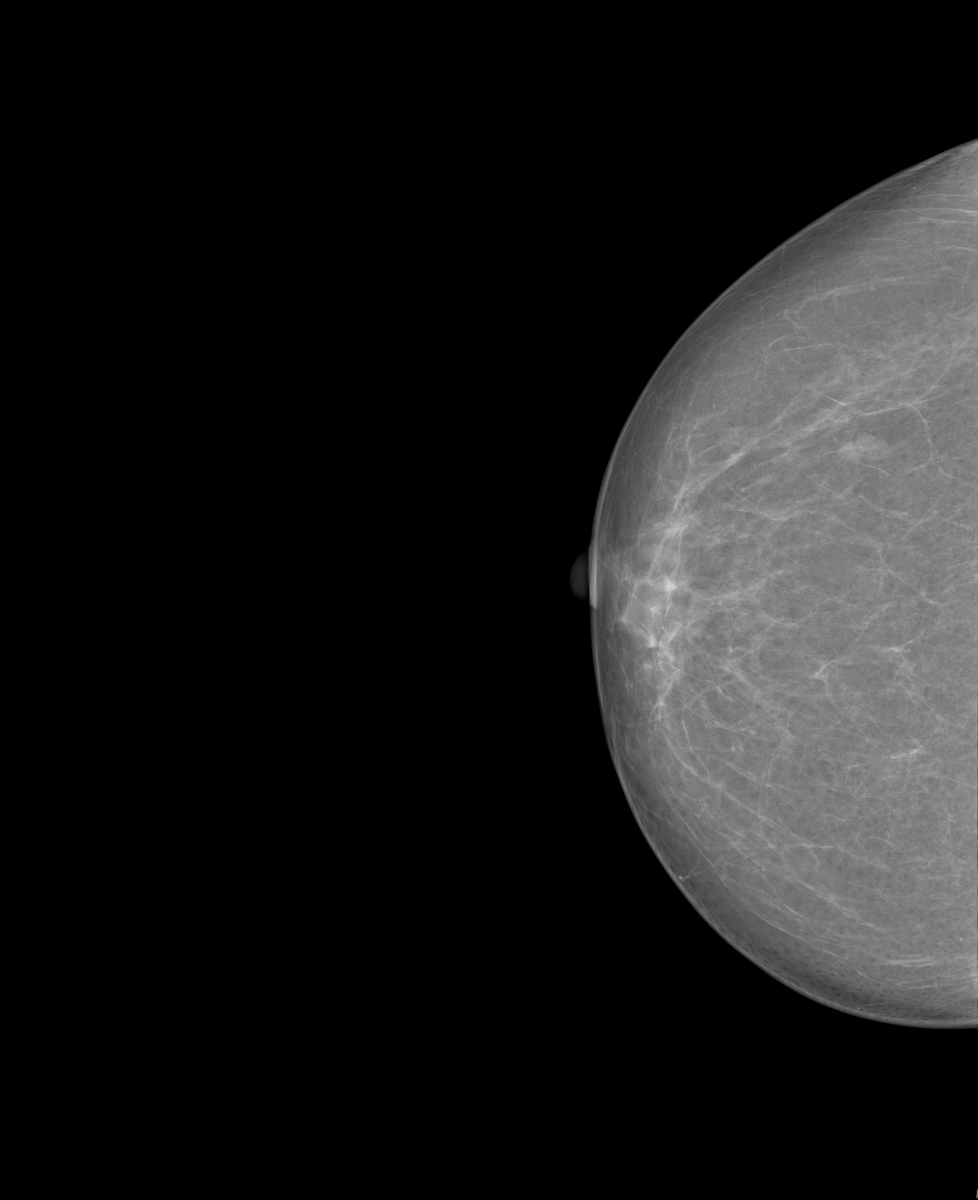
\includegraphics[height = 5cm]{plots/mammogram.png}
    \end{subfigure}
	\begin{subfigure}{4.2 cm}
		\centering
                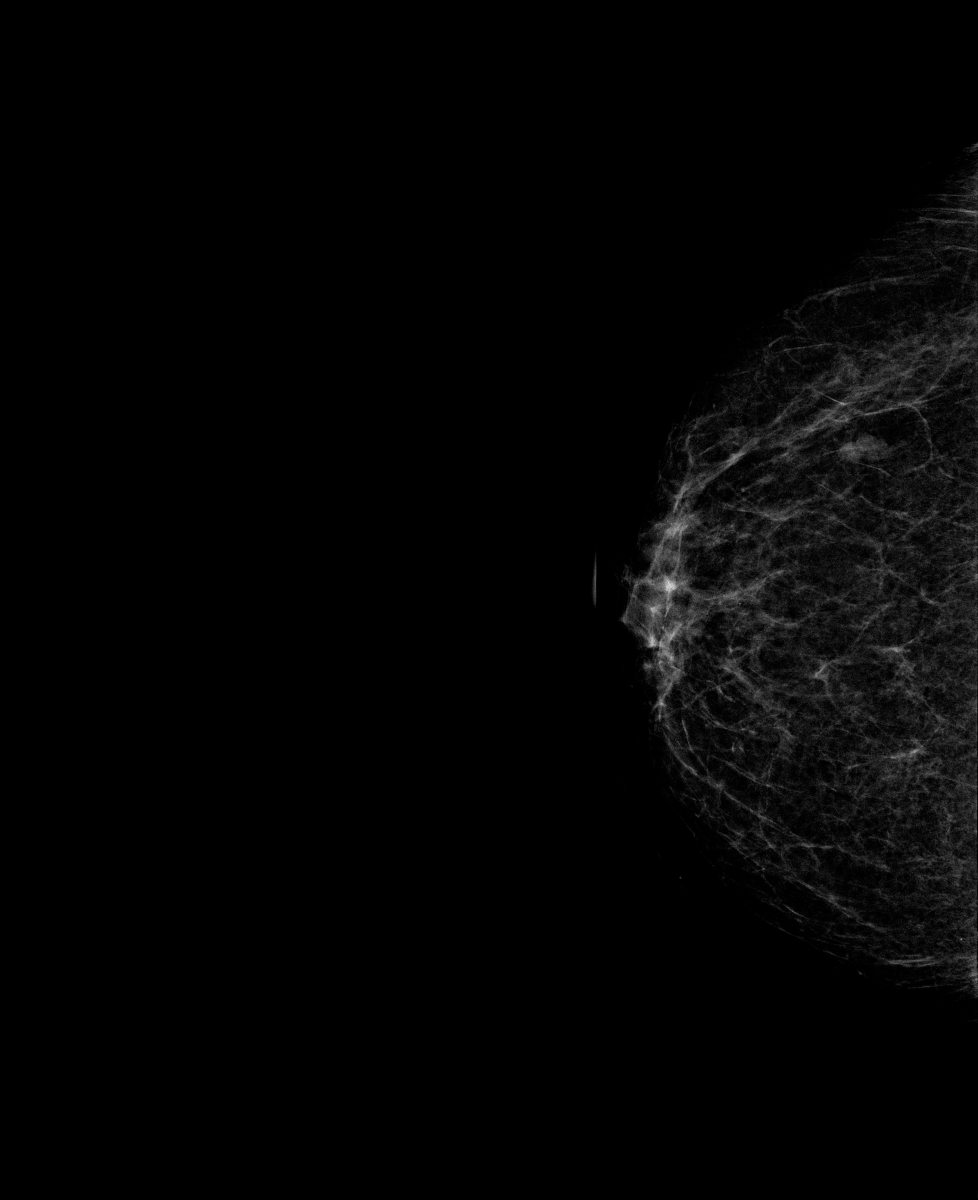
\includegraphics[height = 5cm]{plots/mammogram_enhanced.png}
    \end{subfigure}
	\begin{subfigure}{4.2 cm}
		\centering
                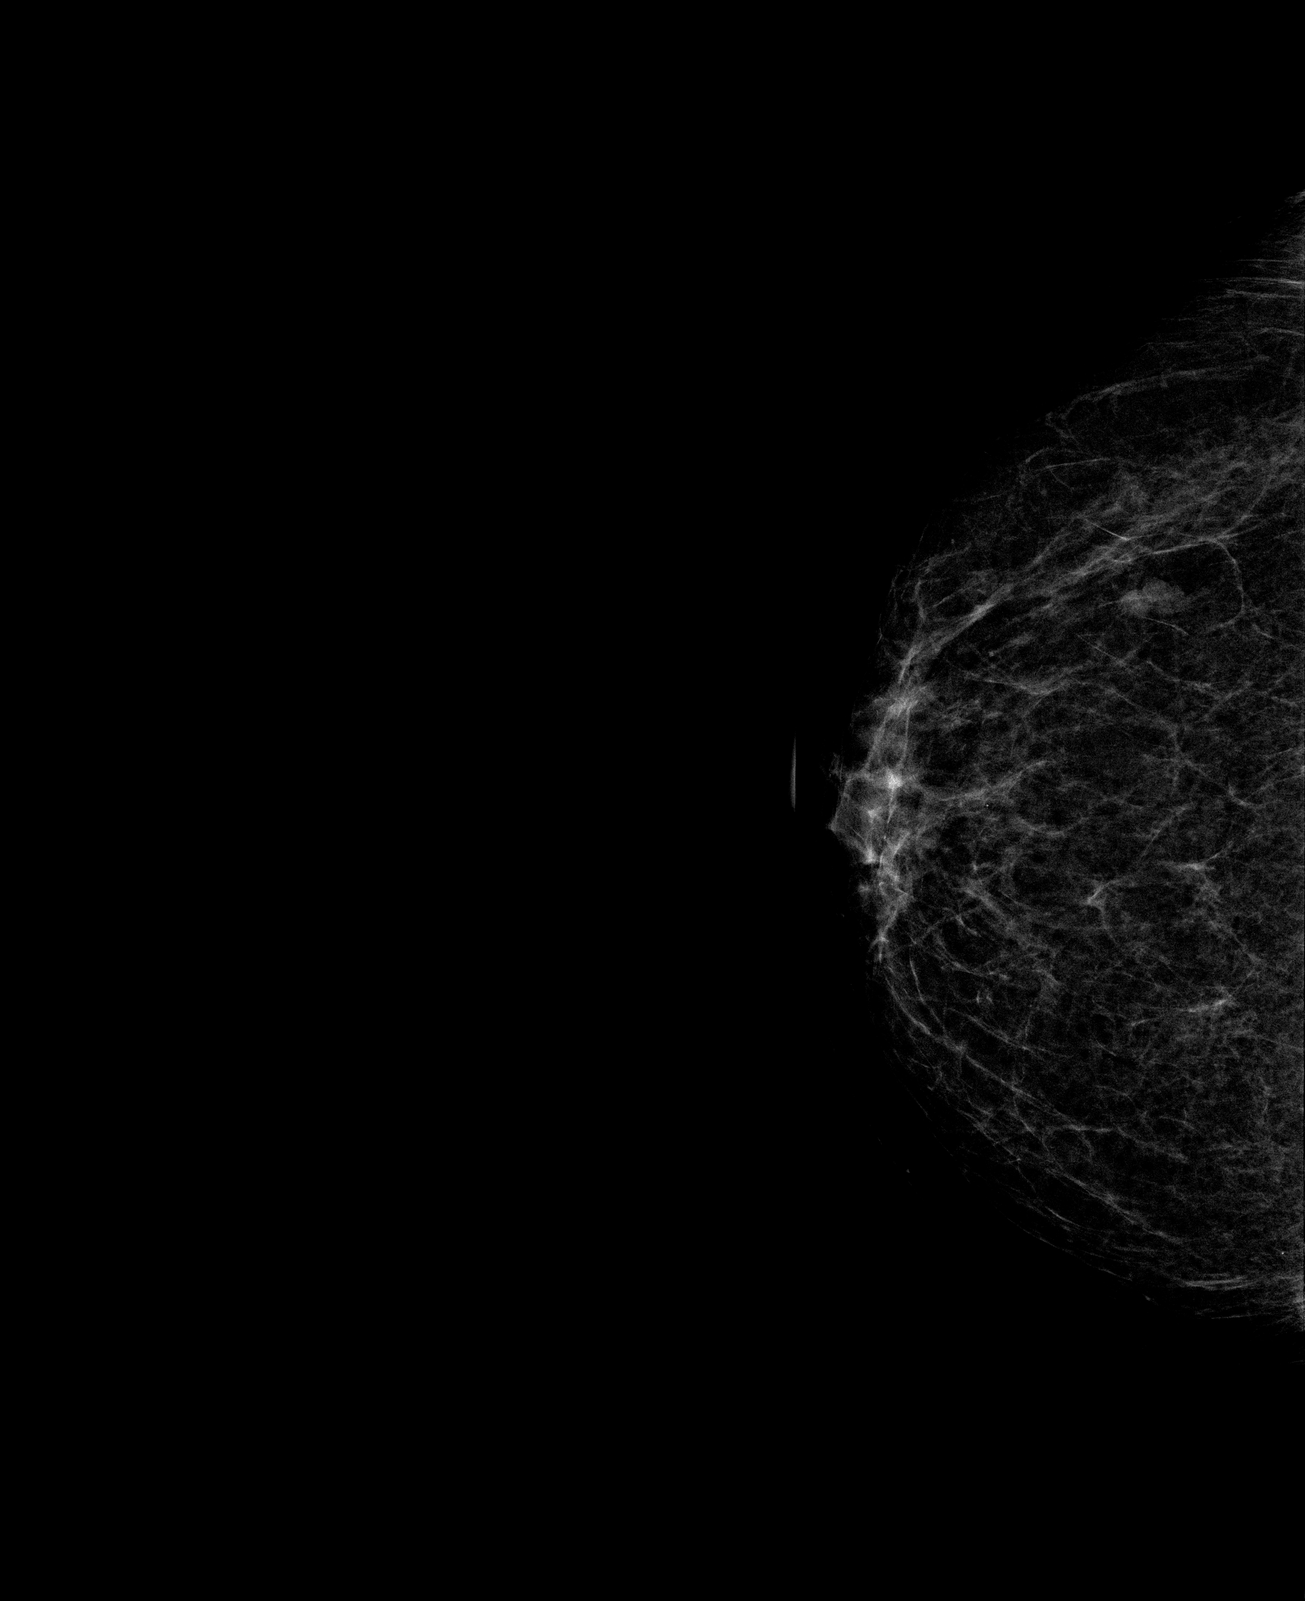
\includegraphics[height = 5cm]{plots/mammogram_resized.png}
    \end{subfigure}
	\begin{subfigure}{2.4 cm}
		\centering
                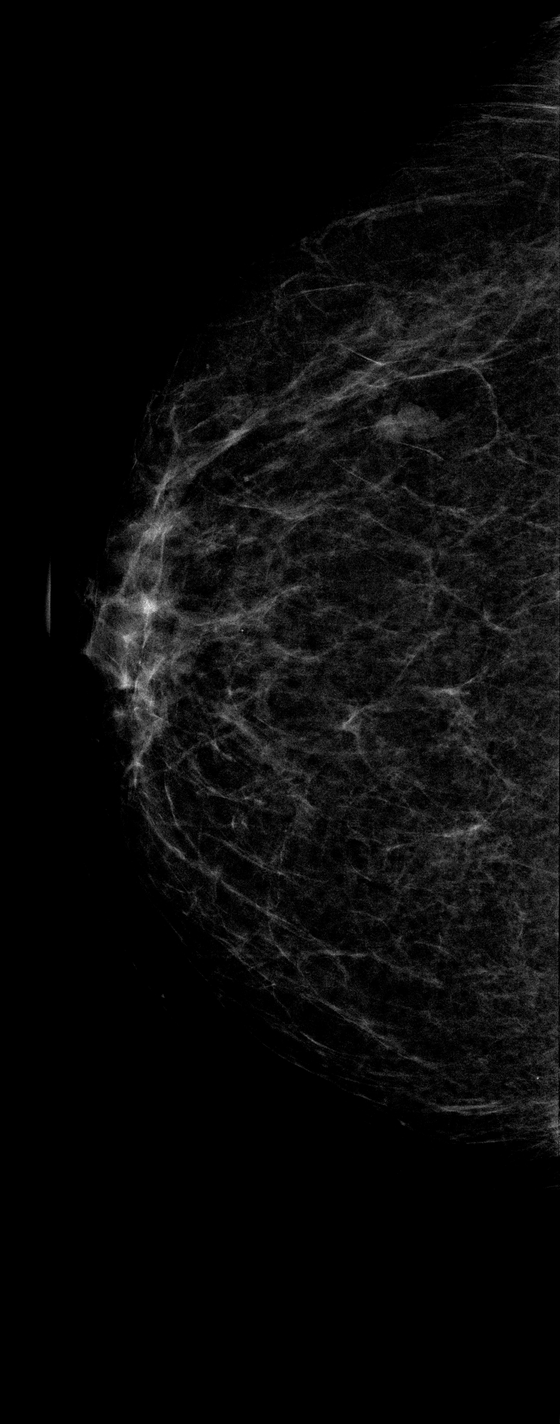
\includegraphics[height = 5cm]{plots/mammogram_v1.png}
    \end{subfigure}
	\\
	\begin{subfigure}{4.2 cm}
		\centering
                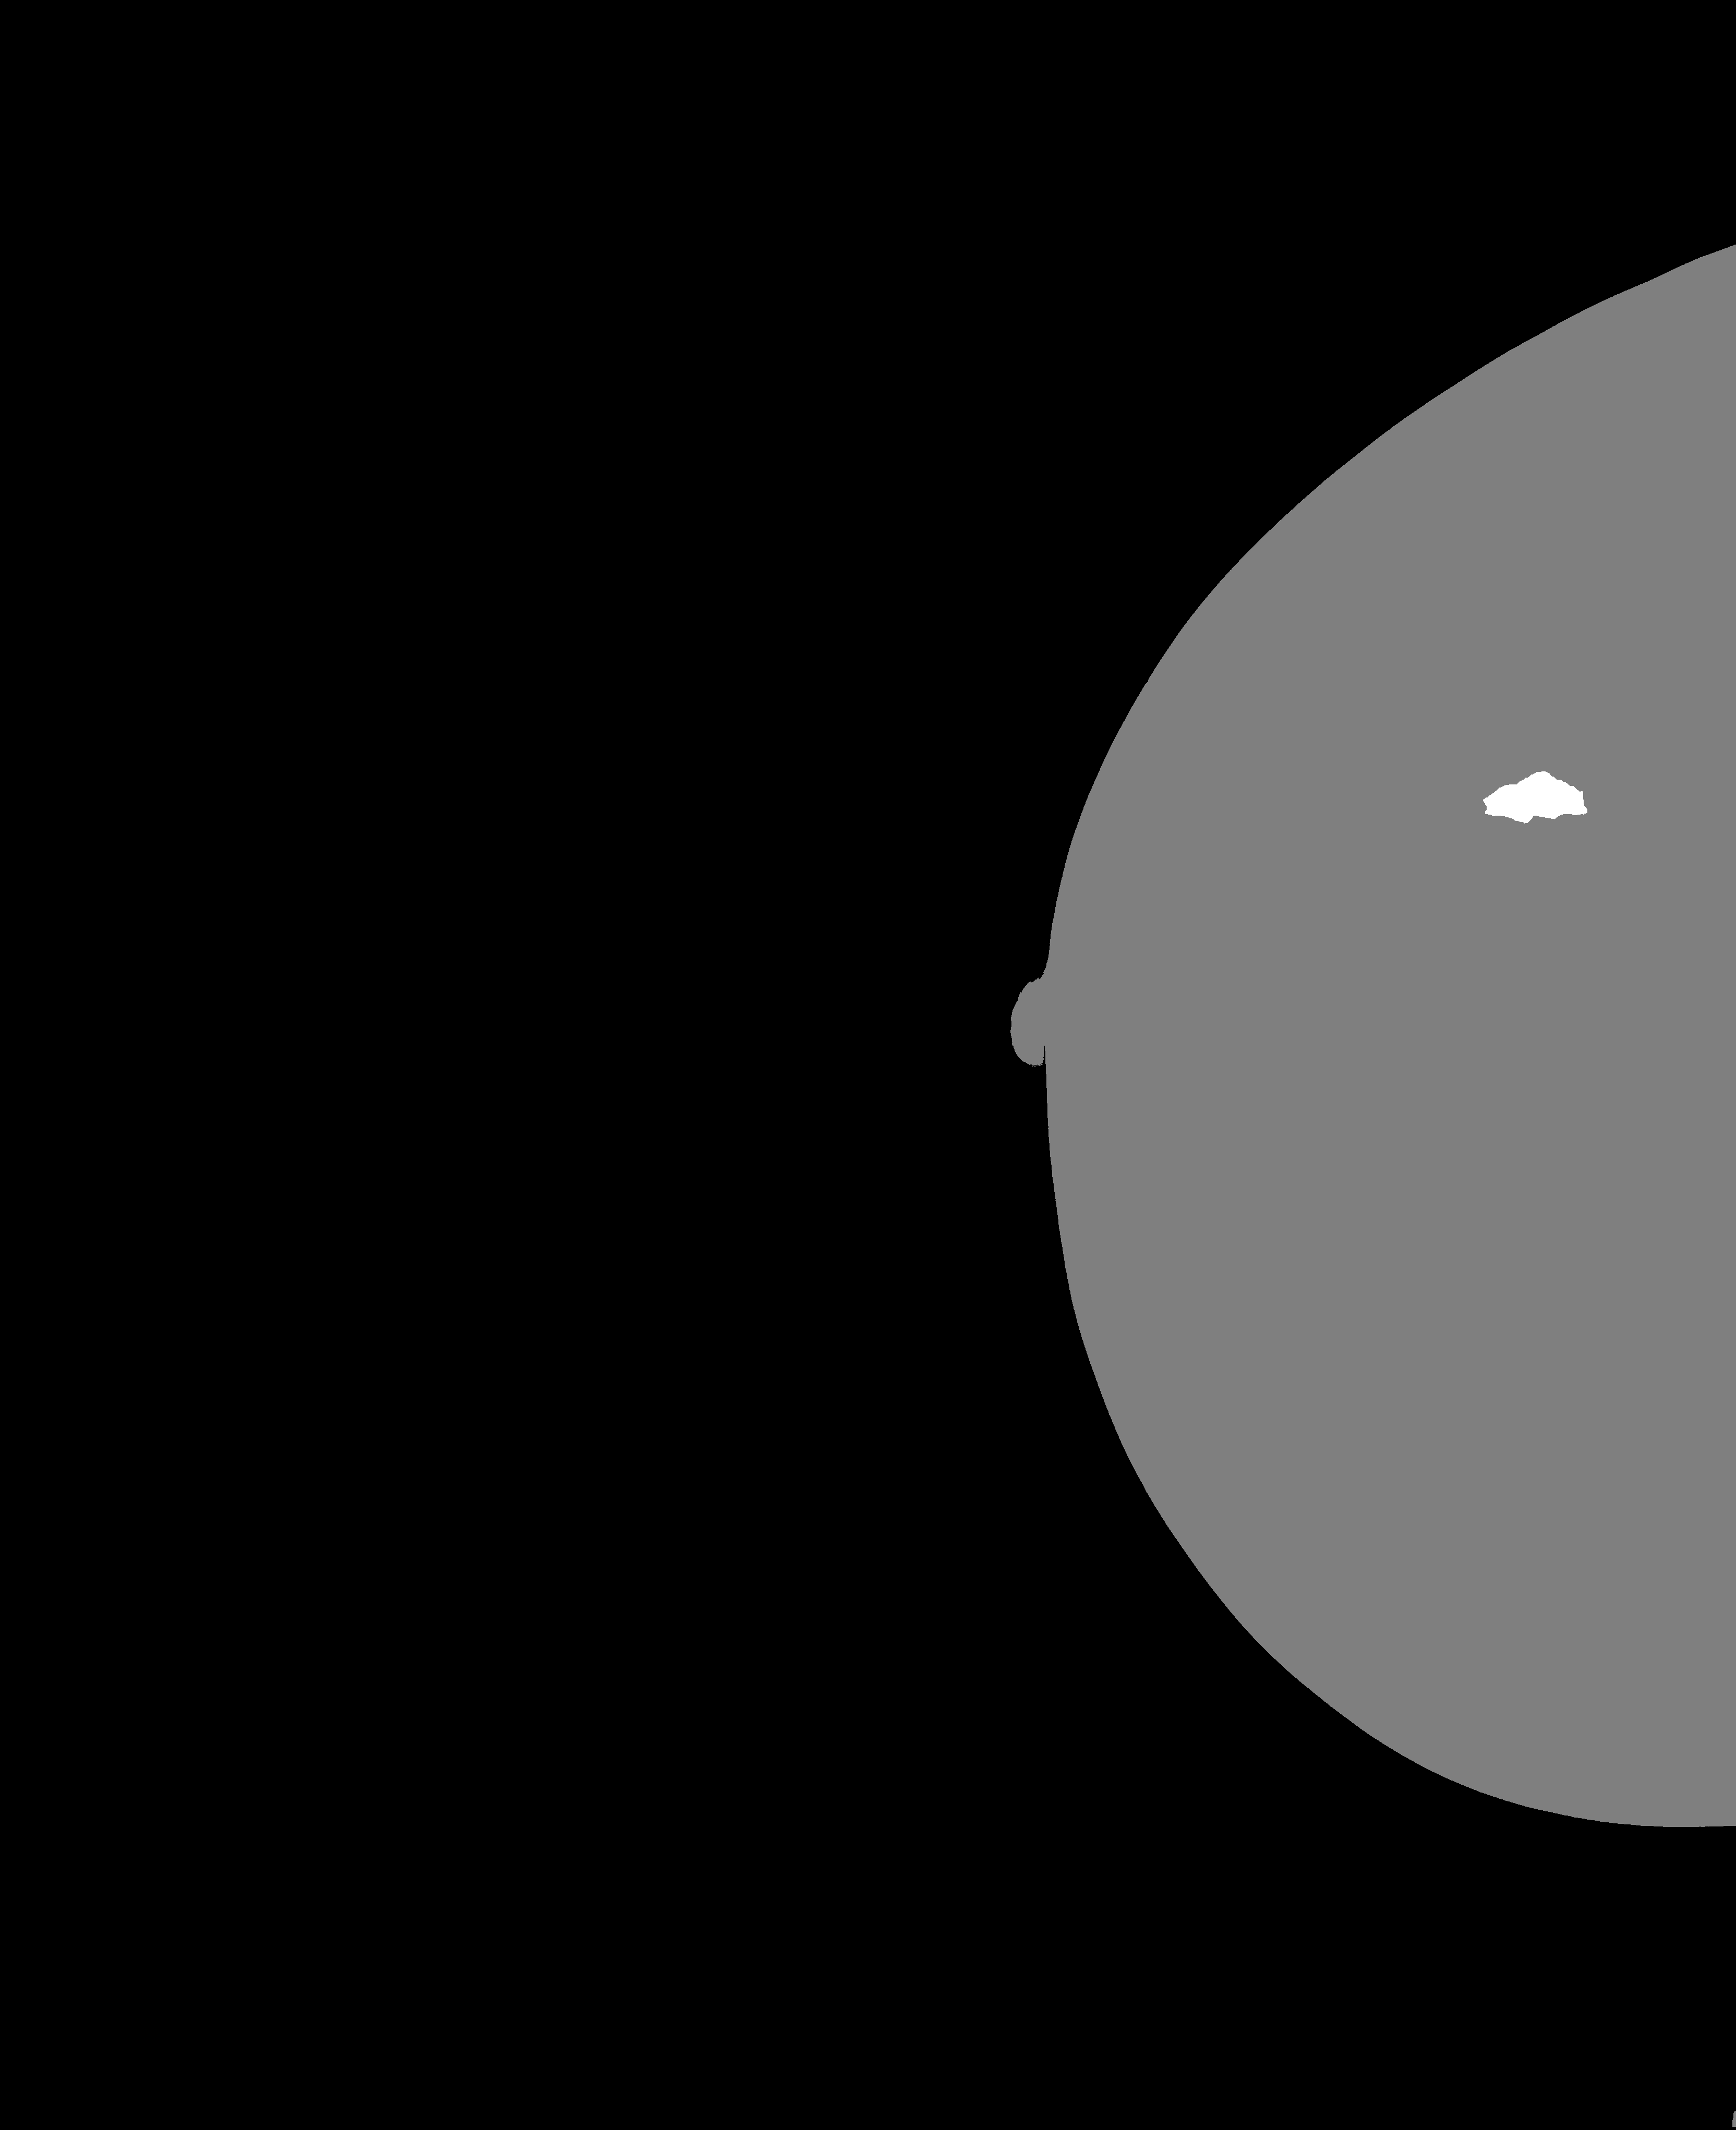
\includegraphics[height = 5cm]{plots/label.png}
		\caption{Original image}
		\label{subfig:Preprocessinga}
    \end{subfigure}
	\begin{subfigure}{4.2 cm}
		\centering
                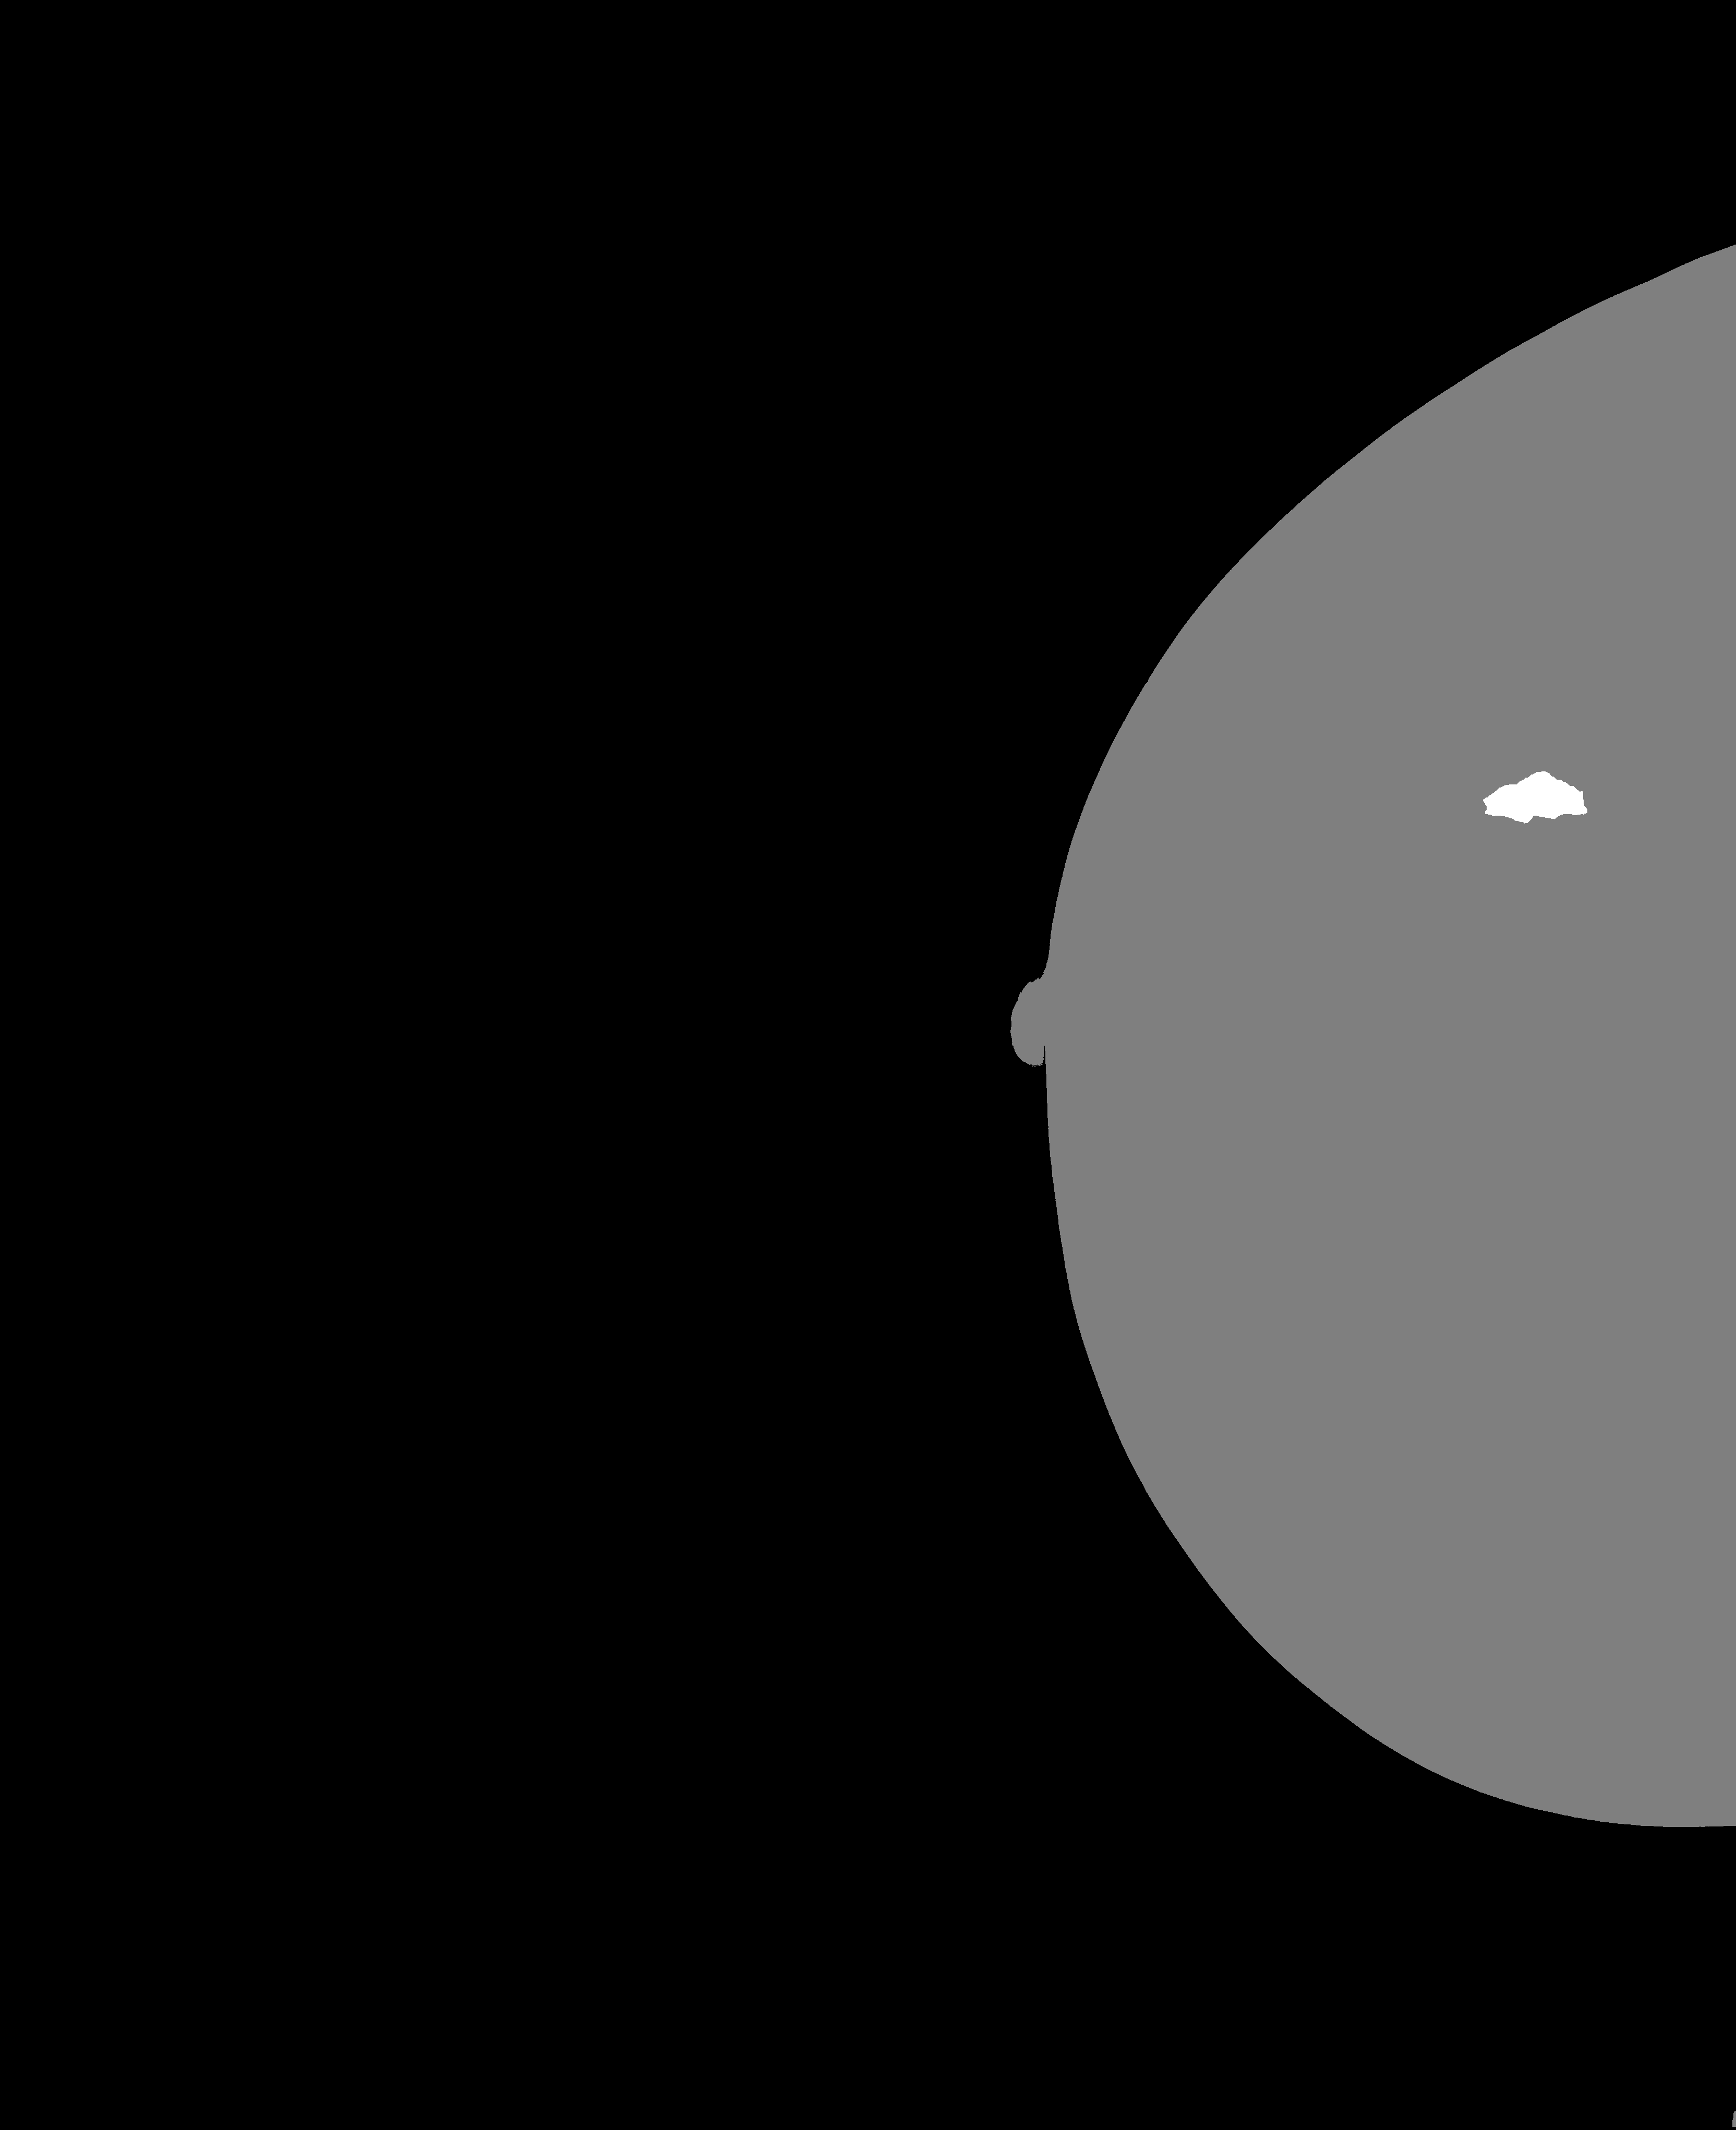
\includegraphics[height = 5cm]{plots/label_enhanced.png}
		\caption{Enhancement}
		\label{subfig:Preprocessingb}
    \end{subfigure}
	\begin{subfigure}{4.2 cm}
		\centering
                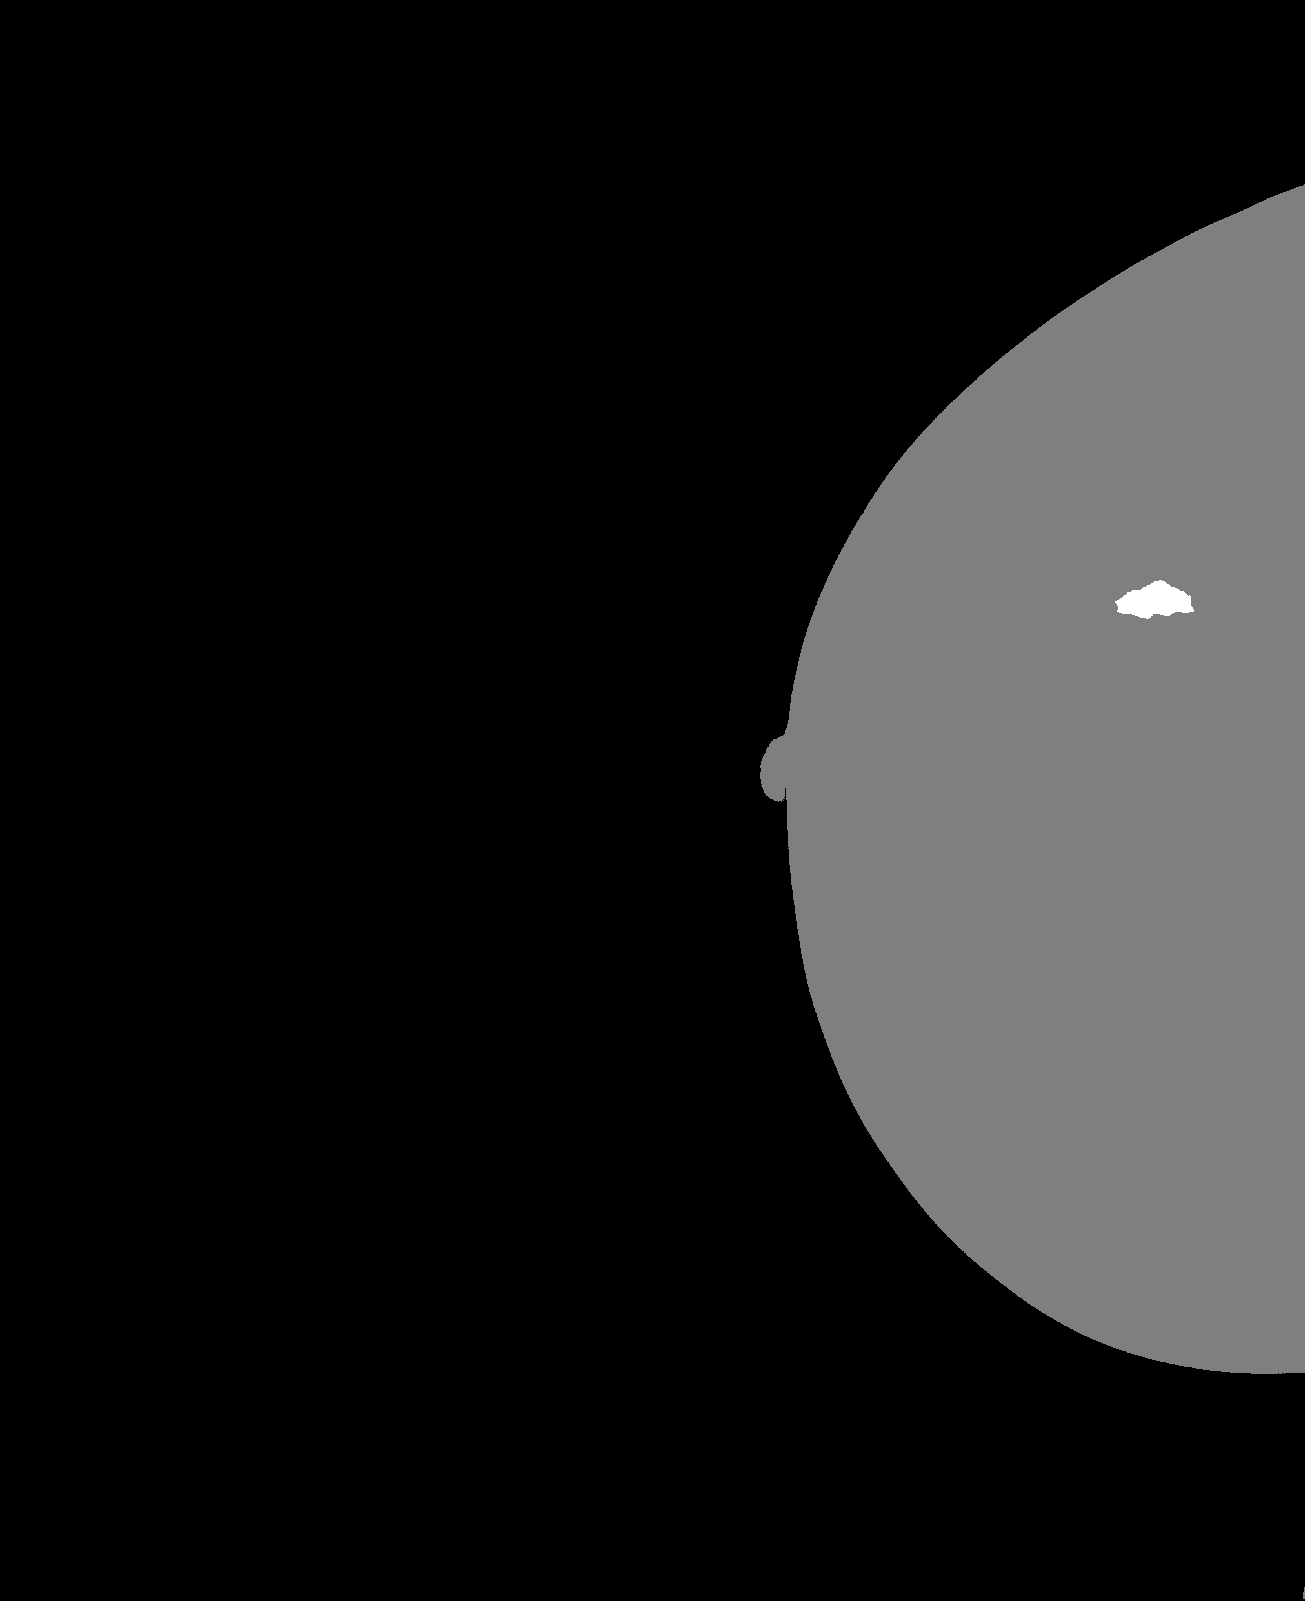
\includegraphics[height = 5cm]{plots/label_resized.png}
		\caption{Downsampling}
		\label{subfig:Preprocessingc}
    \end{subfigure}
	\begin{subfigure}{2.4 cm}
		\centering
		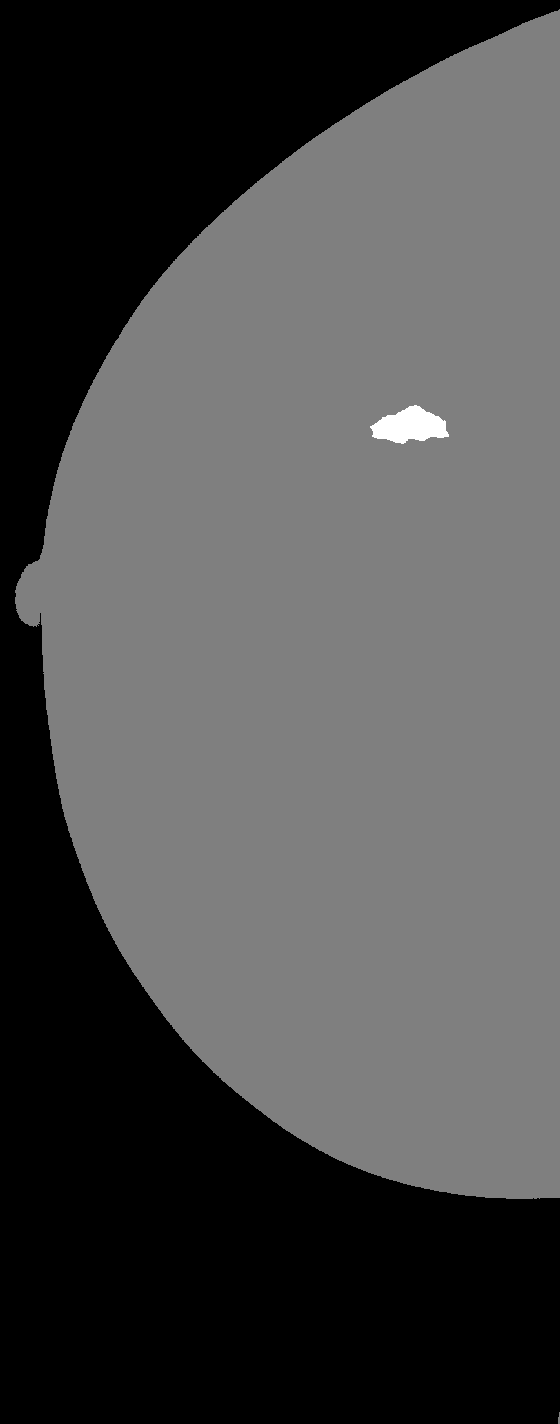
\includegraphics[height = 5cm]{plots/label_v1.png}
		\caption{Final image}
		\label{subfig:Preprocessingd}
    \end{subfigure}
	\caption[Preprocessing pipeline]{A mammogram (top) and its label (bottom) being preprocessed: (1) original images ($4084 \times 3328$), (2) background reduction plus contrast normalization, (3) downsampling and  (4) cropping to delete black spaces ($560 \times 1424$). Augmentation is not shown.}
	 \label{fig:Preprocessing}
% img_108_146_1_RCC.png
\end{figure}
	
\subsection{Data augmentation}
We mirror each image (mammograms and labels) and rotate the original and mirrored version at 0, 90, 180 and 270 degrees to increase our training set by a factor of 8. 
%Mammograms and labels are mirrored and both the original and mirrored version rotated at 0, 90, 180 and 270 degrees to increase our training and validation set by a factor of 8. 
Images in the test set are not augmented. 

This transformations are common when training convolutional networks with small data sets. In principle, the test set should not be augmented as it is a proxy for real data. %In principle it is not neccesary to store the augmented images because they can be easily generated during training but if the disk space is not prohibitive explicitly storing them simplifies training.

%\subsection{Memory compromises} Hopefully not
% Cutting mammograms in 4 or 16 pieces for training would not be that bad, I would have to cut images surrounded with 48 pixels of surrounding regions so the netwrok also sees that and does not see black spaces, then to the output of the network i have to discard a surrounding region of 3 pixels all around to obtain the segmentation of my wanted image: this is exactkly as if training with the big entire image. This if i have no memory, or maybe if i want to change up a bit.

\subsection{Storage}
All mammograms and their respective labels are stored as grayscale 8-bit images preserving their original names (plus a suffix) and folder organization.
% For training, a file enlisting the names of all the images is also generated.
The entire data set before augmentation weights approximately 120 megabytes.


\section{Model 1}
\label{sec:Model1}
We use a simple architecture to have a baseline performance for convolutional networks and test the effect of using a weighted loss function and enhancing the input images.

\subsection{Architecture}
\begin{table}[h!]
	\centering
	\begin{tabular}{lcccccr}
	\hline
	\textbf{Layer} & \textbf{Filter} & \textbf{Stride} & \textbf{Pad} & \textbf{Dilation} & \textbf{Volume} & \textbf{Parameters} \\
	\hline
	\texttt{INPUT}	&- & -	& - & - & $52 \times 52 \times 1$ & -\\
	\texttt{CONV -> RELU}	& $5 \times 5$ & 2 & 2 & 1 & $26 \times 26 \times 32$ & 832\\
	\texttt{CONV -> RELU}	& $3 \times 3$ & 1 & 1 & 1 & $26 \times 26 \times 32$ & 9\,248\\
	\texttt{CONV -> RELU}	& $3 \times 3$ & 2 & 1 & 1 & $13 \times 13 \times 64$ & 18\,496\\
	\texttt{CONV -> RELU}	& $3 \times 3$ & 1 & 1 & 1 & $13 \times 13 \times 64$ & 36\,928\\
	\texttt{CONV -> RELU}	& $3 \times 3$ & 1 & 2 & 2 & $13 \times 13 \times 96$ & 55\,392\\
	\texttt{CONV -> RELU}	& $3 \times 3$ & 1 & 2 & 2 & $13 \times 13 \times 96$ & 83\,040\\
	\texttt{CONV}			& $5 \times 5$ & 1 & 6 & 3 & $13 \times 13 \times 1$ & 2\,401\\
	\texttt{BILINEAR (x4)}	& - & - && - & $52 \times 52 \times 1$ & -\\
	\hline
	\end{tabular}
	\caption[Convolutional network architecture for Experiment 1]{Architecture of the network used for the first experiments. It shows the filter size, stride, padding and dilation in each layer as well as the resulting volume and number of learnable parameters per layer.}
	\label{tab:convNetArchitecture1}
\end{table} % 206 337 params

Each image is whitened (zero-mean centered and divided by its standard deviation) individually before being input. 
The first convolutional layer reduces the spatial dimensions of the input from $52 \times 52$ to $26 \times 26$ to reduce the number of parameters and memory requirements and augment its receptive field. Subsequent convolutional layers preserve the dimensions of its input volume relegating subsampling to pooling layers. 
Finally, the volume is upsampled by a factor of four to recover the dimensions of the original image. The network outputs a heatmap of logits with the same size as the input image.
%We produce a heatmap of logits rather than probabilities to improve numerical stability.

The effective receptive field of the network is $101 \times 101$ pixels , which equates to $2.1 \times 2.1$ cms. This architecture uses 206\,337 parameters. %2 906 681

\subsection{Regularization}
We use l2-norm regularization with $\lambda$ selected using a validation set as explained in Sec.~\ref{subsec:Hyperparameters}.

\subsection{Loss function}
We compute the logistic loss function for each pixel in the produced segmentation and average the loss over pixels in the breast area---background is ignored. This amounts to using a weighted loss function where errors in the breast tissue and masses are weighted by one and those in the background are weighted by zero.

\subsection{Experiments}
We performed three experiments using this architecture:
\subsubsection{Experiment 1.1} 
To obtain a performance baseline, we trained this simple network in minimally processed images, i.e., mammograms without any enhancement.

\subsubsection{Experiment 1.2} 
\label{subsec:Experiment1_2}
To fight the class imbalance due to breast mass pixels being rare in comparison to normal breast tissue pixels, we modify the loss function by weighting errors over masses by fifteen, those over normal breast tissue by one and ignoring those over the background. This forces networks to invest more resources in correctly classifying masses to avoid this costly errors~\cite{Provost2000}. As in the previous experiment, we do not enhance the input.
%This technique balances the total sum of losses from the common class (normal breast tissue) with that of the rare class (breast masses) and is often used to fight class imbalance.

\subsubsection{Experiment 1.3}
In the final experiment, we combine both a weighted loss function and enhanced input images.


\section{Model 2}
\label{sec:Model 2}
We build a complex architecture to test whether we can benefit from the added flexibility.

\subsection{Architecture}
\label{subsec:Architecture1}
%Following recommendations from Section~\ref{sec:PracticalDL}, we define a network with seven convolutional layers and two fully connected layers (Tab.~\ref{tab:convNetArchitecture}). 
We model our architecture on a VGG network~\cite{Simonyan2014}, winner of the 2014 ImageNet competition~(Tab.~\ref{tab:convNetArchitecture1}).
\begin{table}[h]
	\centering
	\begin{tabular}{lccccr}
	\hline
	\textbf{Layer} & \textbf{Filter} & \textbf{Stride} &\textbf{Pad} & \textbf{Volume} & \textbf{Parameters} \\
	\hline
	\texttt{INPUT}	& -	& - & - & $112 \times 112 \times 1$ & -\\
	\texttt{CONV -> Leaky RELU} & $6 \times 6$ & 2 & 2 & $56 \times 56 \times 56$ & 2\,072\\
	\texttt{CONV -> Leaky RELU} & $3 \times 3$ & 1 & 1 & $56 \times 56 \times 56$ & 28\,280\\
	\texttt{MAXPOOL} & $2 \times 2$ & 2 & 0 & $28 \times 28 \times 56$ & -\\
	\texttt{CONV -> Leaky RELU} & $3 \times 3$ & 1 & 1 & $28 \times 28 \times 84$ & 42\,420\\
	\texttt{CONV -> Leaky RELU} & $3 \times 3$ & 1 & 1 & $28 \times 28 \times 84$ & 63\,588\\
	\texttt{MAXPOOL} & $2 \times 2$ & 2 & 0 & $14 \times 14 \times 84$ & -\\
	\texttt{CONV -> Leaky RELU} & $3 \times 3$ & 1 & 1 & $14 \times 14 \times 112$ & 84\,784\\
	\texttt{CONV -> Leaky RELU} & $3 \times 3$ & 1 & 1 & $14 \times 14 \times 112$ & 113\,008\\
	\texttt{CONV -> Leaky RELU} & $3 \times 3$ & 1 & 1 & $14 \times 14 \times 112$ & 113\,008\\
	\texttt{MAXPOOL} & $2 \times 2$ & 2 & 0 & $7 \times 7 \times 112$ & -\\
	\texttt{FC -> Leaky RELU} & $7 \times 7$ & 1 & 3 & $7 \times 7 \times 448$ & 2\,459\,072\\
	\texttt{FC} & $1 \times 1$ & 1 & 0 & $7 \times 7 \times 1$ & 449 \\
	\texttt{BILINEAR (x16)} & - & - & - & $112 \times 112 \times 1$ & -\\
	\hline
	\end{tabular}
	\caption[Selected convolutional network architecture]{Architecture of the network used for experiments. It shows the filter size, stride, padding, resulting volume and number of learnable parameters per layer.}
	\label{tab:convNetArchitecture1}
\end{table}

This network has an effective receptive field of $184 \times 184$ pixels ($2.9 \times 2.9$ cms) and defines $2\,906\,681$ parameters. %2 906 681 %108 752 632 float numbers

\subsection{Regularization}
We use dropout after every leaky ReLU layer with probability 0.9, 0.9, 0.8, 0.8, 0.7, 0.7, 0.7 and 0.6, respectively. We also use l2-norm regularization with $\lambda$ selected using a validation set.

\subsection{Loss function}
As explained in Sec~\ref{subsec:Experiment1_2}, we use a weighted logistic loss function with errors over breast mass pixels weighted by fifteen, over normal breast tissue by one and over the background by zero.

\subsection{Experiments}
We train a single network using input images with no enhancement. Results from this experiment are directly comparable to those in Experiment 1.2 which has the same configuration.


\section{Model 3}
\label{sec:Model3}
To investigate whether negative results are the product of a poorly chosen architecture we designed a different network that is deeper but has fewer parameters than the one used in the previous experiment.

\subsection{Architecture}
We model the architecture on the Residual network~\cite{He2015b}, winner of the 2015 ImageNet competition(Tab~\ref{tab:convNetArchitecture3}).
\begin{table}[h]
	\centering
	\begin{tabular}{lcccccr}
	\hline
	\textbf{Layer} & \textbf{Filter} & \textbf{Stride} & \textbf{Pad} & \textbf{Dilation} & \textbf{Volume} & \textbf{Parameters} \\
	\hline
	\texttt{INPUT}	&- & -	& - & - & $116 \times 116 \times 1$ & -\\
	\texttt{CONV -> LRELU}	& $6 \times 6$ & 2 & 2 & 1 & $58 \times 58 \times 32$ & 1\,184\\
	\texttt{CONV -> LRELU}	& $3 \times 3$ & 1 & 1 & 1 & $58 \times 58 \times 32$ & 9\,248\\
	\texttt{CONV -> LRELU}	& $3 \times 3$ & 2 & 1 & 1 & $29 \times 29 \times 64$ & 18\,496\\
	\texttt{CONV -> LRELU}	& $3 \times 3$ & 1 & 1 & 1 & $29 \times 29 \times 64$ & 36\,928\\
	\texttt{CONV -> LRELU}	& $3 \times 3$ & 1 & 2 & 2 & $29 \times 29 \times 128$ & 73\,856\\
	\texttt{CONV -> LRELU}	& $3 \times 3$ & 1 & 2 & 2 & $29 \times 29 \times 128$ & 147\,584\\
	\texttt{CONV -> LRELU}	& $3 \times 3$ & 1 & 2 & 2 & $29 \times 29 \times 128$ & 147\,584\\
	\texttt{CONV -> LRELU}	& $3 \times 3$ & 1 & 2 & 2 & $29 \times 29 \times 128$ & 147\,584\\
	\texttt{CONV -> LRELU}	& $3 \times 3$ & 1 & 4 & 4 & $29 \times 29 \times 256$ & 295\,168\\
	\texttt{CONV}	& $8 \times 8$ & 1 & 14 & 4 & $29 \times 29 \times 1$ & 16\,385\\
	\texttt{BILINEAR (x4)}		& - & - && - & $116 \times 116 \times 1$ & -\\
	\hline
	\end{tabular}
	\caption[Convolutional network architecture for Experiment 3]{Architecture of the network used for experiments. It shows the filter size, stride, dilation and padding in each layer as well as the resulting volume and number of learnable parameters per layer. \texttt{LRELU} stands for leaky ReLU.}
	\label{tab:convNetArchitecture3}
\end{table}

	 %We replace pooling by strided convolutions~\cite{Szegedy2014} or dilated convolutions~\cite{Chen2015}. Input images are whitened independently and passed to the network that produces the predicted segmentation. Because the volume is downsampled only by a factor of four before the upsampling layer, we are able to produce fine-grained segmentations.
This 10-layer architecture uses 894\,017 parameters and has a receptive field size of $228 \times 228$, equivalent to a $3.6 \times 3.6$ cm area.
	
\subsection{Regularization}
We use l2-norm regularization ($\lambda$ chosen using a validation set) and dropout after RELU layers with probabilities 0.9, 0.9, 0.8, 0.8, 0.7, 0.7, 0.7, 0.7 and 0.6.

\subsection{Loss function}
We use a weighted logistic loss function with errors over breast masses weighted by 0.9, errors over normal breast tissue weighted by 0.1 and errors over background weighted by zero. 

\subsection{Experiments}
We train a single network in enhanced mammograms. Results from this experiment can be compared to those in Experiment 1.3.


\section{Training}
We offer details about the learning stage of our experiments.
% including hardware, software and optimization algorithms and other implementation notes.

\subsection{Hardware}
%Training neural networks is computationally intensive and requires equipment with powerful GPUs. 
We performed our experiments in 30 machines with the following specification:
\begin{table}[h]
	\centering
	\begin{tabular}{cp{3.8cm}p{1.8cm}cc}
	\hline
	\textbf{Location}	& \textbf{GPU}	& \textbf{CPU} &\textbf{HD}	& \textbf{RAM}\\
	\hline
	%Personal	& Nvidia NVS 5400M \newline 96 cores, 1GB, compute capability 2.1 & i5-3210M \newline 2.5GHz & 57 GB & 4 GB\\
	A4-401 & Nvidia Quadro K620 \newline 384 cores, 2GB, compute capability 5.0 & i5-4570 \newline 3.2GHz	& 240 GB & 8 GB\\
	\hline
	\end{tabular}
	\caption{Available hardware for experiments}
\end{table}

Each computer was used independently to train networks (not distributed). Although we designed our models to be small enough to fit in the GPU memory, big images surpassed this limit causing errors; thus, we decided to train our networks only with the CPU. Training times ranged from 1 to 1.5 hours per 1000 examples.

\subsection{Software}
Models were implemented and trained using TensorFlow (v.11)~\cite{Abadi2015}. Tools for image retrieval, augmentation, evaluation and similar tasks were implemented in Python 3.
Code, as well as some trained models, are freely accesible at: \url{github.com/ecobost/cnn4brca}.

\subsection{Initialization}
Weights for the incoming connections to a unit are drawn from a normal distribution with zero mean and $\sqrt{2/n_{in}}$ standard deviation where $n_{in}$ is the number of connections. Biases are initialized to zero.

\subsection{Hyperparameter search}
\label{subsec:Hyperparameters}
We fit the learning rate and regulatization parameter simultaneously using random sampling. For each fold independently, we train 20 networks for five epochs (6\,520 examples) and select the best ($\alpha$, $\lambda$) combination using 20\% of the fold as a validation set. We use sensitivity at one false positive per image as performance metric.

\subsection{Optimization}
We use ADAM ($\beta_1 = 0.9$, $\beta_2 = 0.995$ and $\epsilon = 10^{-6}$) for optimization.
%, i.e., we perform stochastic gradient descent (with momentum and per-parameter adaptive learning rate).
Each parameter update uses the information from only a single training example but thanks to the loss function being a weighted average over all pixels in the image, gradients are as rich as if we were performing mini-batch gradient descent with a batch composed of all image patches for which the network produced a prediction.

We trained the final model for all experiments for 30 epochs (49\,200 examples). No early stopping was performed.
% Any early stopping thing here


\section{Evaluation}
We describe how we evaluate our results.

\subsection{Post-processing}
We aim to evaluate convolutional networks as a single end-to-end segmentation model;
%component in an end-to-end segmentation task;
thus, we choose to use the produced heatmaps without any post-processing. However, adding post-processing to our best performing architecture will certainly improve results and remains as a viable future endeavor.% In any case, having a strong network to start with is needed to produce good results.

% Options:
% uncorrected threshold: Select a threshold, take that as segementation
% Cluster-extent correction: Delete thresholds that are under a number of pixels 
% or whose total probability is less than a desired number. Needs this number
% Threshold-free cluster enhancement (module 29 in introduction to fmri): Same as aove but withouth a cluster (?)
% Number of clusters per image: do threshold-free enhancement where the metric is to 
% leave only the most promising cluster
% Conditional random fields (CRF): Work quite well. Python implementation of CRF: https://pystruct.github.io/auto_examples/image_segmentation.html Here is another take: http://www.robots.ox.ac.uk/~szheng/CRFasRNN.html Any look fine.

\subsection{Segmentation}
We generate a segmentation by setting each pixel whose value was zero in the original mammogram to background (0), each non-background pixel whose logit is greater than a threshold to breast mass (255) and any remaining pixel to normal breast tissue (127) (Fig.~\ref{fig:Post-processing}).

\begin{figure}[h]
	\centering
	\begin{subfigure}{0.2\textwidth}
		\centering
                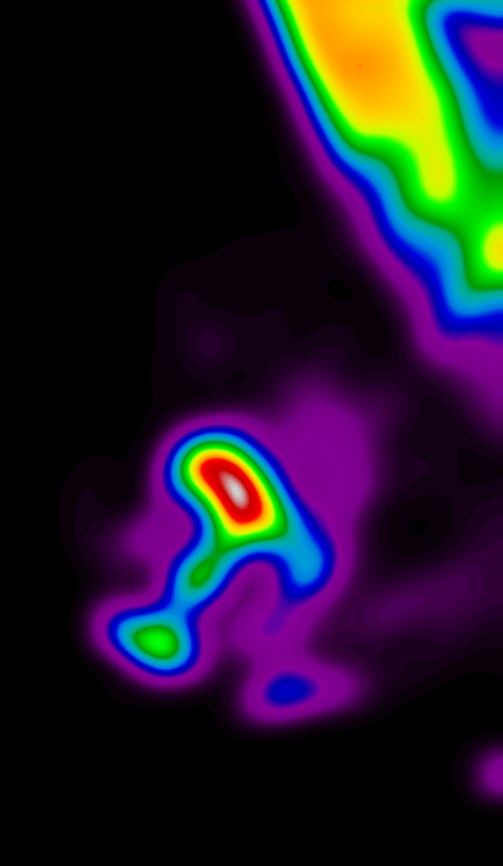
\includegraphics[width=\textwidth]{plots/probs.png}
         \caption{Prediction}
	\end{subfigure}
	\quad
	\begin{subfigure}{0.2\textwidth}
		\centering
                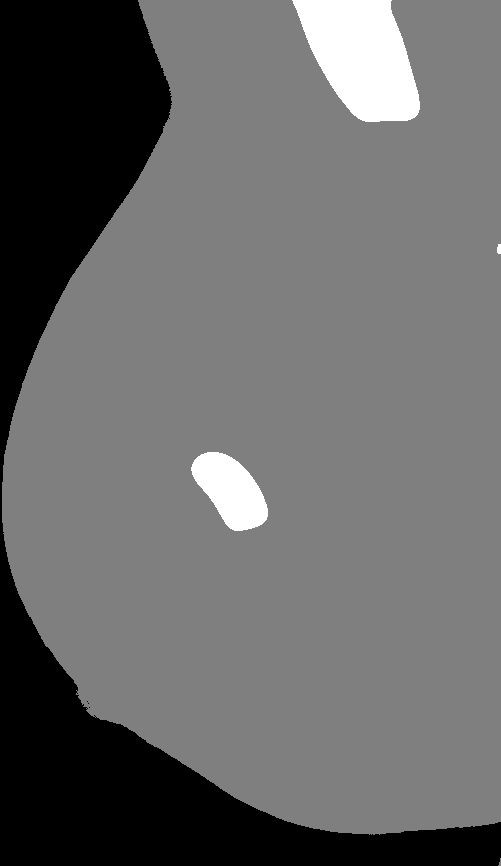
\includegraphics[width=\textwidth]{plots/segmentation.png}
         \caption{Segmentation}
	\end{subfigure}
	\caption[Post-processing pipeline]{Heatmap of probabilities and segmentation produced by assigning all background to black and thresholding at probability 0.5.}
	 \label{fig:Post-processing}
\end{figure}
% Using the validation set, we compute the IOU for different thresholds and select the one that produces the best result. The final segmentation is generated by setting each pixel whose value was zero in the original mammogram to background (0), each non-background pixel whose logit is greater than the threshold to breast mass (255) and any remaining pixel to normal breast tissue (127).

\subsection{Metrics}
We use five-fold cross-validation and the free-response ROC curve to evaluate our models. We count a breast mass as a true positive if a blob in the segmentation covers at least 10\% of its area. To avoid any bias, we compute the number of false positives per image only in the images without a breast mass~\cite{Chakraborty2013}. Furthermore, we force the number of false positives in an image to be non-decreasing for lower, i.e., laxer thresholds.


\section{Summary}
Mammograms from the BCDR-D01 database were enhanced, resized and divided to obtain our data set. A simple architecture (6 layers, 206K parameters) was used for the first experiments, one of which used a weighted loss function to tackle class imbalance. Two more sophisticated architectures based on the VGG network (9 layers, 2.9M parameters) and residual networks (10 layers, 0.9M parameters) were used for the following experiments. We performed hyperparameter search to fine tune the learning rate and regularization parameter of each network; other hyperparameters were set manually. Networks were written in TensorFlow and optimized using ADAM. We use five-fold cross-validation for evaluation. We report the FROC curve for the final models.
